\documentclass[a4paper,12pt]{article}
\usepackage[lmargin=30mm,rmargin=30mm,tmargin=25mm,bmargin=25mm,showframe]{geometry}
\usepackage{mathptmx}% http://ctan.org/pkg/mathptmx

\usepackage[T1]{fontenc}
\usepackage{textcomp}
\usepackage{unicode-math}

\usepackage[estonian]{babel}
%\usepackage[none]{hyphenat}

%\setmathfont[Scale=0.85]{Lucida Bright Math OT}
%\setmathfont{TeX Gyre Pagella Math}


\usepackage{fancyhdr}
\fancypagestyle{FirstPage}{\fancyhf{}\renewcommand{\headrulewidth}{0pt}\fancyfoot[C]{Tallinn 2017}}

\renewcommand*\contentsname{\vskip 60pt\centering Sisukord}
\renewcommand*\listfigurename{\vskip 60pt\centering Jooniste loetelu}

\usepackage{biblatex}
\bibliography{thesis}

\usepackage{hyperref}

\usepackage[figure,table]{totalcount}

%\linespread{1.4}
%\renewcommand{\baselinestretch}{1.5}

\setlength{\parindent}{0pt}
\setlength{\parskip}{12pt}

\usepackage{titlesec}

% http://tex.stackexchange.com/questions/299969/titlesec-loss-of-section-numbering-with-the-new-update-2016-03-15
\usepackage{etoolbox}
\makeatletter
\patchcmd{\ttlh@hang}{\parindent\z@}{\parindent\z@\leavevmode}{}{}
\patchcmd{\ttlh@hang}{\noindent}{}{}{}
\makeatother

%\titleformat{\section}[block]{\color{blue}\Large\bfseries\filcenter}{}{1em}{}
\titlespacing*{\section}{0pt}{60pt}{18pt}
\titlespacing*{\subsection}{0pt}{24pt}{12pt}
% III tase: kiri 14pt, lõiguvahe enne ja pärast 12pt

\usepackage{underscore}
\usepackage{listings}
\lstdefinelanguage{agda}{
  morekeywords={abstract,constructor,data,field,
    forall,hiding,import,in,infix,infixl,infixr,let,
    module,mutual,open,postulate,primitive,Prop,
    private,public,quoteGoal,quoteTerm,quote,record,
    renaming,rewrite,Set,syntax,unquote,using,where,with},
  keywordstyle=\bfseries,
  mathescape=true,
  basicstyle=\fontsize{11}{11}\selectfont\sffamily,
  %comment=[l]{--},
  morecomment=[s]{\{-}{-\}},
  escapechar=\&
}
\lstset{language=agda}

\usepackage{float}
\floatstyle{boxed} 
\restylefloat{figure}

\usepackage{caption}
\captionsetup[figure]{name=Joonis}

\usepackage{tikz}

\renewcommand{\labelitemi}{$\smblksquare$}

\usepackage{setspace}
\begin{document}
\onehalfspacing

% ------------------------------------------------------------
  \begin{center}
    \textsc{tallinna tehnikaülikool}\\
    Infotehnoloogia teaduskond\\
    Arvutiteaduse instituut\\
    \vfill
    
    Tõnn Talvik 132619IAPM
    \vskip 3em 
    \LARGE\textsc{efekti analüüside ja nendel põhinevate programmiteisenduste sertifitseerimine}\\
    \normalsize\vskip 4em 
    Magistritöö\\
    \vskip 4em    
  \end{center}
  
  \begin{flushright}
    \begin{tabular}{ r l }
      Juhendaja:& Tarmo Uustalu\\
      & Professor \\
    \end{tabular}
    \vfill
  \end{flushright}
  
  \thispagestyle{FirstPage}
  \clearpage
  \setcounter{page}{2}
% ------------------------------------------------------------

\section*{\vskip 60pt\centering Autorideklaratsioon}

Kinnitan, et olen koostanud antud lõputöö iseseisvalt ning seda ei ole kellegi teise poolt varem kaitsmisele esitatud. Kõik töö koostamisel kasutatud teiste autorite tööd, olulised seisukohad, kirjandusallikatest ja mujalt pärinevad andmed on töös viidatud.

Autor: Tõnn Talvik

8. mai 2017
\clearpage

\section*{\vskip 60pt\centering Annotatsioon}
[tekst]
         
Lõputöö on kirjutatud eesti keeles ning sisaldab teksti [lehekülgede arv töö põhiosas] leheküljel, [peatükkide arv] peatükki, \totalfigures\ joonist, [tabelite arv] tabelit.
\clearpage

\section*{\vskip 60pt\centering Abstract\\
Certification of effect analysis and program transformations based on the analysis}
[text]
The thesis is in Estonian and contains [pages] pages of text, [chapters] chapters, \totalfigures\ figures, [tables] tables.
\clearpage

\tableofcontents
\clearpage

\listoffigures
\clearpage







\section{Sissejuhatus}

% background and motivation?
Taust: efektid ja monaadid. Moggi, Benton, Katsumata.

% https://courses.cs.ttu.ee/pages/Problem_Statement

Töö eesmärgiks on realiseerida sõltuvate tüüpidega programmeerimiskeeles Agda idee tõestus taseme
raamistu efektide analüüsiks ja nendele põhinevateks programmiteisendusteks.
Samas raamistus peab saama näidata, et need analüüsid ja teisendused on korrektsed.
% Sissejuhatuses tutvustab autor töö teemat, töö eesmärke, lahendatavat probleemistikku,
% andes samuti ülevaate töö ülesehitusest. Sissejuhatuses kirjeldatakse ka töö
% lähtetingimused, alamülesanded ja vajadusel ka täiendavad nõuded (vt jaotist 2.4 ).

% Lõputöös peab sisalduma selge lõpetaja poolt lahendatava ülesande püstitus.

% Magistritöös esitatakse lahendatava ülesande püstitus töö sissejuhatuses, kattes järgmised punktid:
% - töös lahendatavad küsimused ja lähtetingimused,
% - eritingimused, mida on rakendatud ülesande lahendamisel/ülesande püstitamisel.

% Rigor
rääkida Agdast ja tõestustest

% Reproducibility
Töö käigus valminud lähtekood on tulemuste reprodutseerimiseks allalaetav aadressilt \url{https://github.com/tonn-talvik/msc}.
Lähtekoodi kompileerimiseks on kasutatud Agda versiooni 2.5.1.1 koos standardteegi versiooniga 0.12.
Mainitud tarkvarapaketid on tasuta installeeritavad Ubuntu 16.04 LTS jt varamutest.


\clearpage

\section{Erandid}

Selles peatükis vaadeldakse keele laiendust eranditega. 
Baaskeeleks on tüübitud lambda-arvutus koos tõeväärtuste, naturaalarvude ja korrutistega.
Järgnevates alapeatükkides defineeritakse selline keel Agdas,
viiakse läbi tüübituletus koos efekti analüüsiga,
määratakse hästi tüübitud avaldiste semantika
ning tuuakse mõned optimeerivate programmiteisenduste näited.
Ühtlasi näidatakse analüüsi ja teisenduste korrektsust.

\subsection{Eranditega keel}

Vastastikku defineeritud väärtus- ja arvutustüübid on toodud joonisel \ref{fig:exc.types}.
Lubatud väärtustüübid VType on naturaalarvud, tõeväärtused, teiste väärtustüüpide korrutised ja tüübitud lambda-arvutused.
Arvutustüüpideks on efektiga E annoteeritud väärtustüübid. Efekt E on defineeritud alapeatükis \ref{ssec:exc.grading}.
\begin{figure}
  \begin{lstlisting}
mutual
  data VType : Set where
    nat : VType
    bool : VType
    _$∏$_ : VType →  VType → VType
    _$⟹$_ : VType →&\ &CType →&\ &VType

  data CType : Set where
    _/_ : E → VType → CType
  \end{lstlisting}
  \caption{Eranditega keele tüübid.}
  \label{fig:exc.types}
\end{figure}


Vastastikku defineeritud väärtus- ja arvutustermid on toodud joonisel \ref{fig:exc.raw}.
% pragmatics
Termide konstruktorite nimetamisel on kasutatud suurtähti vältimaks võimalikke nimekonflikte Agda standard funktsioonidega.
Järgnevalt on selgitatud väärtustermi vTerm konstruktorite tähendust.
\begin{itemize}
  \item TT ja FF koostavad vastavalt tõeväärtused tõene ja väär.
  \item ZZ koostab naturaalarvu 0 ja konstruktor SS oma argumendist järgneva naturaalarvu.
  \item $⟨$_,_$⟩$ koostab oma argumentide paari e. korrutise.
  \item FST ja SND koostavad vastavalt argumendina antud korrutise esimese ja teise projektsiooni.
  \item VAR koostab De Bruijn'i indeksiga määratud muutuja.
  \item LAM on funktsiooni abstraktsioon, seejuures funktsiooni parameetri väärtustüüp on eksplitsiitselt annoteeritud. Funktsiooni kehaks on arvutusterm.
\end{itemize}

\begin{figure}
  \begin{lstlisting}
mutual
  data vTerm : Set where
    TT FF : vTerm
    ZZ : vTerm
    SS : vTerm → vTerm
    $⟨$_,_$⟩$ : vTerm →  vTerm → vTerm
    FST SND : vTerm → vTerm
    VAR : $ℕ$ →  vTerm
    LAM : VType → cTerm → vTerm

  data cTerm : Set where
    VAL : vTerm → cTerm
    FAIL : VType → cTerm
    TRY_WITH_ : cTerm → cTerm → cTerm
    IF_THEN_ELSE_ : vTerm → cTerm → cTerm → cTerm
    _&\$&_ : vTerm → vTerm → cTerm
    PREC : vTerm → cTerm → cTerm → cTerm
    LET_IN_ : cTerm → cTerm → cTerm

  \end{lstlisting}
  \caption{Eranditega keele väärtus- ja arvutustermid.}
  \label{fig:exc.raw}
\end{figure}

Järgnevalt on selgitatud arvutustermi cTerm konstruktorite (jn \ref{fig:exc.raw}) tähendust ja vastavas arvutuses kätketud efekti.
\begin{itemize}
  \item VAL tähistab õnnestunud arvutust, seejuures arvutuse tulemuseks on väärtustermiga antud konstruktori argument.
  \item FAIL tähistab arvutuse, mille väärtustüüp on eksplitsiitselt annoteeritud, ebaõnnestumist.
  \item TRY_WITH_ on arvutuse erandikäsitleja: kogu arvutuse tulemuseks on esimese argumendiga antud termi arvutus, kui see õnnestub, vastasel korral aga teise argumendiga antud termi arvutus.
  \item IF_THEN_ELSE_ on valikuline arvutus: vastavalt väärtustermi tõeväärtusele on tulemuseks kas esimese (tõene haru) või teise (väär haru) arvutustermiga antud arvutus.
  \item _\$_ on esimese väärtustermiga antud funktsiooni rakendamine teise väärtustermiga antud väärtusele, kusjuures rakendamise efektiks on funktsioonis peituv efekt.
  \item PREC on primitiivne rekursioon, mille sammude arv on määratud väärtustermi argumendiga. Esimene arvutusterm vastab rekursiooni baasile ja teine sammule, kusjuures sammuks on akumulaatori ja sammuloenduri parameetritega funktsioon. Kogu arvutuse efekt vastab kõigi osaarvutuste järjestikku sooritamisele.
  \item LET_IN_ lisab esimese arvutustermiga antud väärtuse teise arvutustermi kontekstis esimeseks muutujaks. Arvutuse efekt vastab osaarvutuste järjestikku sooritamisele.
\end{itemize}

\begin{figure}
  \begin{lstlisting}
ADD : vTerm
ADD = LAM nat
          (VAL (LAM nat
                    (PREC (VAR 0)
                          (VAL (VAR 1))
                          (VAL (SS (VAR 0))))))

ADD-3-and-4 : cTerm
ADD-3-and-4 = LET ADD &\$& (SS (SS (SS ZZ)))
              IN VAR 0 &\$& (SS (SS (SS (SS ZZ))))

BAD-ONE : cTerm
BAD-ONE = ZZ &\$& TT
  \end{lstlisting}
  \caption{Näidisavaldised eranditega keeles.}
  \label{fig:exc.raw.ex1}
\end{figure}

Joonisel \ref{fig:exc.raw.ex1} on toodud kahe naturaalarvu liitmise funktsioon väärtustermina ADD
ning naturaalarvude 3 ja 4 liitmine arvutustermina ADD-3-and-4.
Lisaks on toodud näide arvutustermist BAD-ONE, mida annab konstrueerida,
kuid mis ei oma sisu: naturaalarvu null ei saa rakendada tõeväärtusele tõene.
Sellised halvasti tüübitud termid tuvastatakse tüübituletusega (alaptk \ref{ssec:exc.inference}).

\subsection{Erandite gradeering} \label{ssec:exc.grading}

Erandite efekti hinnang Exc on toodud joonisel \ref{fig:exc.exc}: konstruktor err vastab arvutuse ebaõnnestumisele, konstruktor ok arvutuse õnnestumisele ja konstruktor errok arvutusele, mille kohta pole teada, kas see õnnestub või mitte.

Efektide korrutamine _·_ (jn \ref{fig:exc.exc}) vastab arvutuste järjestikule sooritamisele. 

Hinnangu Exc konstruktorid moodustavad järgneva võre:
\begin{center}
  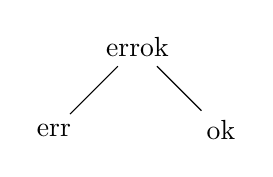
\begin{tikzpicture}[node distance=1.5cm]
    \node (top) at (0,0) {errok};
    \node [below left  of=top] (left)  {err};
    \node [below right of=top] (right) {ok};
    \draw (top) -- (left);
    \draw (top) -- (right);
  \end{tikzpicture}
\end{center}
Hinnangute järjestusseos _$⊑$_ on toodud joonisel \ref{fig:exc.exc}. See seos on refleksiivne $⊑$-refl. Transitiivsuse $⊑$-trans tõestus seisneb argumentide kuju juhtumi analüüsil. Transitiivsuse seost on võimalik kodeerida järjestusseose konstruktorina, kuid see pole otstarbekas, kuna hilisemates tõestuses tekib sellest täiendavad juhtumid, mida peab analüüsima.
\begin{figure}
  \begin{lstlisting}
data Exc : Set where
  err : Exc
  ok : Exc
  errok : Exc
  
_·_ : Exc → Exc → Exc
ok · e = e
err · e = err
errok · err = err
errok · ok = errok
errok · errok = errok

data _&$⊑$&_ : Exc → Exc → Set where
  &$⊑$&-refl : {e : Exc} → e &$⊑$& e
  err&$⊑$&errok : err &$⊑$& errok
  ok&$⊑$&errok : ok &$⊑$& errok
  
&$⊑$&-trans : {e e' e'' : Exc} → e &$⊑$& e' → e' &$⊑$& e'' → e &$⊑$& e''
&$⊑$&-trans &$⊑$&-refl q = q
&$⊑$&-trans err&$⊑$&errok &$⊑$&-refl = err&$⊑$&errok
&$⊑$&-trans ok&$⊑$&errok &$⊑$&-refl = ok&$⊑$&errok
  \end{lstlisting}
  \caption{Erandite efektid, nende korrutamine ja efektide järjestatus.}
  \label{fig:exc.exc}
\end{figure}



\subsubsection{Järjestatud monoid}
Järjestatud monoid: järjestatuse transitiivsus, korrutamine, korrutamise assotsiatiivsus, monotoonsus, vasak ühik, parem ühik.

\subsubsection{Gradeeritud monaad}
T, $\eta$, lift, sub, mlaw1,2,3, 
\subsubsection{Alamtüübid}

\subsection{Tüübituletus ja efekti analüüs} \label{ssec:exc.inference}

Joonisel \ref{fig:exc.refined} on toodud vastastikku defineeritud rafineeritud väärtus- ja arvutustermid.
Termid on parametriseeritud kontekstiga $Γ$ ning indekseeritud vastavalt väärtus- ja arvutustüüpidega.
Kontekst Ctx on defineeritud kui väärtusttüüpide list.
\begin{figure}
  \begin{lstlisting}
Ctx = List VType

mutual
 data VTerm (&$Γ$& : Ctx) : VType → Set where
   TT FF : VTerm &$Γ$& bool
   ZZ : VTerm &$Γ$& nat
   SS : VTerm &$Γ$& nat → VTerm &$Γ$& nat
   $⟨$_,_$⟩$ : {&$σ$& &$σ'$& : VType} →
           VTerm &$Γ$& &$σ$& → VTerm &$Γ$& &$σ'$& → VTerm &$Γ$& (&$σ$& &$∏$& &$σ'$&)
   FST : {&$σ$& &$σ'$& : VType} → VTerm &$Γ$& (&$σ$& &$∏$& &$σ'$&) → VTerm &$Γ$& &$σ$&
   SND : {&$σ$& &$σ'$& : VType} → VTerm &$Γ$& (&$σ$& &$∏$& &$σ'$&) → VTerm &$Γ$& &$σ'$&
   VAR : {&$σ$& : VType} → &$σ$& &$∈$& &$Γ$& → VTerm &$Γ$& &$σ$&
   LAM : (&$σ$& : VType) {&$τ$& : CType} →
         CTerm (&$σ$& &$∷$& &$Γ$&) &$τ$& → VTerm &$Γ$& (&$σ$& &$⟹$& &$τ$&)
   VCAST : {&$σ$& &$σ'$& : VType} → VTerm &$Γ$& &$σ$& → &$σ$& &$≤$&V &$σ'$& → VTerm &$Γ$& &$σ'$&

 data CTerm (&$Γ$& : Ctx) : CType → Set where
   VAL : {&$σ$& : VType} → VTerm &$Γ$& &$σ$& → CTerm &$Γ$& (ok / &$σ$&)
   FAIL : (&$σ$& : VType) → CTerm &$Γ$& (err / &$σ$&)
   TRY_WITH_ : {e e' : E} {&$σ$& : VType} → CTerm &$Γ$& (e / &$σ$&) →
               CTerm &$Γ$& (e' / &$σ$&) → CTerm &$Γ$& (e &$⊹$& e' / &$σ$&)
   IF_THEN_ELSE_ : {e e' : E} {&$σ$& : VType} → VTerm &$Γ$& bool →
     CTerm &$Γ$& (e / &$σ$&) → CTerm &$Γ$& (e' / &$σ$&) → CTerm &$Γ$& (e &$⊔$& e' / &$σ$&)
   _&\$&_ : {&$σ$& : VType} {&$τ$& : CType} →
         VTerm &$Γ$& (&$σ$& &$⟹$& &$τ$&) → VTerm &$Γ$& &$σ$& → CTerm &$Γ$& &$τ$&
   PREC : {e e' : E} {&$σ$& : VType} → VTerm &$Γ$& nat →
          CTerm &$Γ$& (e / &$σ$&) → CTerm (&$σ$& &$∷$& nat &$∷$& &$Γ$&) (e' / &$σ$&) →
          e · e' &$⊑$& e → CTerm &$Γ$& (e / &$σ$&)
   LET_IN_ : {e e' : E} {&$σ$& &$σ'$& : VType} → CTerm &$Γ$& (e / &$σ$&) →
            CTerm (&$σ$& &$∷$& &$Γ$&) (e' / &$σ'$&) → CTerm &$Γ$& (e · e' / &$σ'$&)
   CCAST : {e e' : E} {&$σ$& &$σ'$& : VType} → CTerm &$Γ$& (e / &$σ$&) →
           e / &$σ$& &$≤$&C e' / &$σ'$& → CTerm &$Γ$& (e' / &$σ'$&)
  \end{lstlisting}
  \caption{Eranditega keele rafineeritud termid.}
  \label{fig:exc.refined}
\end{figure}




\begin{figure}
  \begin{lstlisting}
  infer-vtype : (&$Γ$& : Ctx) → vTerm → Maybe VType
  infer-vtype &$Γ$& TT = just bool
  infer-vtype &$Γ$& FF = just bool
  infer-vtype &$Γ$& ZZ = just nat
  infer-vtype &$Γ$& (SS t) with  infer-vtype &$Γ$& t
  ... | just nat = just nat
  ... | _        = nothing
  infer-vtype &$Γ$& $⟨$ t , t' $⟩$ with infer-vtype &$Γ$& t | infer-vtype &$Γ$& t'
  ... | just $σ$ | just $σ'$ = just ($σ ∏ σ'$)
  ... | _      | _       = nothing
  infer-vtype &$Γ$& (FST t) with infer-vtype &$Γ$& t
  ... | just (&$σ$& ∏ _) = just &$σ$&
  ... | _            = nothing
  infer-vtype &$Γ$& (SND t) with infer-vtype &$Γ$& t
  ... | just (_ ∏ &$σ'$&) = just &$σ'$&
  ... | _             = nothing
  infer-vtype &$Γ$& (VAR x) with x <? &$Γ$&
  infer-vtype &$Γ$& (VAR x) | yes p = just (lkp &$Γ$& (from$ℕ≤$ p))
  infer-vtype &$Γ$& (VAR x) | no ¬p = nothing
  infer-vtype &$Γ$& (LAM &$σ$& t) with infer-ctype (&$σ$& &$∷$& &$Γ$&) t
  ... | just &$τ$& = just (&$σ$& ⟹ &$τ$&)
  ... | _      = nothing
  \end{lstlisting}
  \caption{Eranditega keele väärtustüüpide tüübituletus.}
  \label{fig:exc.infer-vtype}
\end{figure}

\begin{figure}
  \begin{lstlisting}
  infer-ctype : (&$Γ$& : Ctx) → cTerm → Maybe CType
  infer-ctype &$Γ$& (VAL x) with infer-vtype &$Γ$& x
  ... | just &$σ$& = just (ok / &$σ$&)
  ... | _      = nothing
  infer-ctype &$Γ$& (FAIL &$σ$&) = just (err / &$σ$&)
  infer-ctype &$Γ$& (TRY t WITH t') with infer-ctype &$Γ$& t | infer-ctype &$Γ$& t'
  ... | just &$τ$& | just &$τ'$& = &$τ$& ⊹C &$τ'$&
  ... | _      | _       = nothing
  infer-ctype &$Γ$& (IF x THEN t ELSE t') with infer-vtype &$Γ$& x | infer-ctype &$Γ$& t | infer-ctype &$Γ$& t'
  ... | just bool | just &$τ$& | just &$τ'$& = &$τ$& ⊔C &$τ'$&
  ... | _         | _      | _       = nothing
  infer-ctype &$Γ$& (f &\$& t) with infer-vtype &$Γ$& f | infer-vtype &$Γ$& t
  infer-ctype &$Γ$& (f &\$& t) | just (&$σ$& ⟹ &$τ$&) | just &$σ'$& with &$σ'$& ≤V? &$σ$&
  infer-ctype &$Γ$& (f &\$& t) | just (&$σ$& ⟹ &$τ$&) | just &$σ'$& | yes _ = just &$τ$&
  infer-ctype &$Γ$& (f &\$& t) | just (_ ⟹ _) | just _  | no  _ = nothing
  infer-ctype &$Γ$& (f &\$& t) | _             | _       = nothing
  infer-ctype &$Γ$& (PREC x t t') with infer-vtype &$Γ$& x
  infer-ctype &$Γ$& (PREC x t t') | just nat with infer-ctype &$Γ$& t
  infer-ctype &$Γ$& (PREC x t t') | just nat | just (e / &$σ$&) with infer-ctype (&$σ$& &$∷$& nat &$∷$& &$Γ$&) t'
  infer-ctype &$Γ$& (PREC x t t') | just nat | just (e / &$σ$&) | just (e' / &$σ'$&) with e · e' &$⊑$&? e | &$σ$& ≡V? &$σ'$&
  infer-ctype &$Γ$& (PREC x t t') | just nat | just (e / &$σ$&) | just (e' / &$σ'$&) | yes _ | yes _ = just (e / &$σ$&)
  infer-ctype &$Γ$& (PREC x t t') | just nat | just (_ / _) | just (_  / _ ) | _     | _      = nothing
  infer-ctype &$Γ$& (PREC x t t') | just nat | just (_ / _) | _ = nothing
  infer-ctype &$Γ$& (PREC x t t') | just nat | _ = nothing
  infer-ctype &$Γ$& (PREC x t t') | _ = nothing
  infer-ctype &$Γ$& (LET t IN t') with infer-ctype &$Γ$& t 
  infer-ctype &$Γ$& (LET t IN t') | just (e / &$σ$&) with infer-ctype (&$σ$& &$∷$& &$Γ$&) t'
  infer-ctype &$Γ$& (LET t IN t') | just (e / &$σ$&) | just (e' / &$σ'$&) = just (e · e' / &$σ'$&)
  infer-ctype &$Γ$& (LET t IN t') | just (_ / _) | _              = nothing
  infer-ctype &$Γ$& (LET t IN t') | _            = nothing
  \end{lstlisting}
  \caption{Eranditega keele arvutustüüpide tüübituletus.}
  \label{fig:exc.infer-ctype}
\end{figure}


\subsection{Semantika}
aoeu
\subsection{Optimisatsioonid}
aeoust haoseu th

\clearpage

\section{Mitte-deterministlik keel}
aseo huasousato usaoheu s
_f_ : a → b\[
∀X [ ∅ ∉ X ⇒ ∃f:X ⟶  ⋃ X\ ∀A ∈ X (f(A) ∈ A )λ ∀ ∃ ⟦ ⟪ · ⊔ ⊓ Γ ρ ε  ⊑   ¬ ≡ ≢ ≤ ≰ ∏ ⇒  ℕ ]\]
\begin{figure}
  \begin{lstlisting}
  private
  data _$⊑$_ : Exc →  Exc → Set where
    $⊑$-refl : {e : Exc} →  e $⊑$ e
    err$⊑$errok : err $⊑$ errok
    ok$⊑$errok : ok ⊑ errok
$λ ∀ ∃ ⟦ ⟧ ⟪ ⟫ · ⊔ ⊓ Γ ρ ε   ¬ ≡ ≢ ≤ ≰ ∏ ⇒ \_  ℕ $
  {-
  data Exc : Set where
    err : Exc
    ok : Exc -- kommentaar 
    errok : Exc
  -}
  \end{lstlisting}
  \caption{Erandite andmetüübi konstruktorid.}
\end{figure}

This is obvious \cite{Benton2016}. \cite{Katsumata2014}

\clearpage

\section{Võimalikud edasiarendused}

- muteeritava oleku laiendused\\
- mittedeterminismi teine gradeering nd0,1,01,1+,N ja selle optimisatsioonid (pure-lambda-hoist, dead-computation)

\clearpage

\section{Kokkuvõte}
Kokkuvõttes esitab autor töö põhieesmärgi, vastused sissejuhatuses püstitatud
küsimustele, toob välja töö olulisemad tulemused ja järeldused.

\clearpage

\renewcommand{\baselinestretch}{1.15}
\fontsize{11}{11}\selectfont
\printbibliography[title={\vskip 60pt\centering Kasutatud kirjandus}]

\end{document}
